% Предустановленные пакеты:
%   texlive-full
% Команда для сборки:
%   latexmk -pdf -bibtex -latexoption="-file-line-error -synctex=1 -interaction=nonstopmode -shell-escape" $fullname

% \documentclass[10pt,twoside]{geodmanual}
\documentclass[10pt,twoside]{extreport}

\usepackage[utf8]{inputenc}
\usepackage[russian]{babel}
\usepackage[OT1]{fontenc}
\usepackage{amsmath}
\usepackage{amsfonts}
\usepackage{amssymb}
\usepackage{makeidx}
\usepackage{graphicx}
\usepackage{hyperref}
\usepackage{enumitem}
\usepackage[left=2cm,right=2cm,top=2cm,bottom=2cm]{geometry}

\title{pyGrav}
\author{roman}

% \manualVersion{\ShowRepoVersion{}}

% \orgFullName{}
% \orgShortName{}
% \divName{}
% \depName{}

% \manualType{Руководство пользователя}
% \manualYear{2023}
% \manualCity{Астана}
% \def \pathtotitlepic {figures/a10.png}

\includeonly{
  chapters/overview,
  chapters/quick_start,
  chapters/pygrav_functions,
  chapters/test_case,
  chapters/code_structure,
  chapters/acquisition_protocol,
  chapters/least_square_inversion_and_error_propagation,
  chapters/installing_external_programs,
}

\newcommand{\pg}{\textbf{\textsf{pyGrav}}}

\begin{document}

\maketitle
\tableofcontents

\chapter[Обзор]{Обзор}
\label{overview}

\pg{} \cite{a10-063_new_instrument_data_report} предназначен для покадровых исследований
гравитации а также для обработки данных о микрогравитации Пользователь может
выбрать между графическим пользовательским интерфейсом (GUI) или классическими
скриптами на Python, вызвав функции pyGrav для обработки данных: поправки на
приливы и атмосферные явления, выбор данных и корректировку дрейфа. Код с
открытым исходным кодом, написан на Python 2.7 и соответствует
объектно-ориентированной схеме, которая позволяет быстро внедрять новые функции
/ опции. В настоящее время формат файла Scintrex CG5 ASCII доступен только для
чтения , но любой другой формат может быть легко добавлен в процедуры чтения
pyGrav. Ключевые моменты кратко излагаются ниже:
\begin{itemize}
    \item Обеспечьте единый интерфейс для различных этапов обработки
    (исправления, выбор данных, корректировка дрейфа, двойные различия ...),
    вместо того, чтобы беспокоиться об управлении различными конкретными
    программами с соответствующими форматами файлов ввода / вывода.
    
    \item Обеспечьте уникальный и простой в использовании интерфейс для выбора
    данных, как с графическим, так и с табличным отображением, а также
    автоматические критерии выбора для ускорения обработки.
    
    \item Написан на языке Python 2.7 с открытым исходным кодом, также может
    использоваться для переноса других программ (таких как MCGRAVI для
    компенсации сети или ETERNA PREDICT для вычисления синтетических приливов).
    
    \item Написан в объектно-ориентированном стиле, подходящем для данных о
    микрогравитации, для которых четко определены объекты с определенными
    свойствами / функциями и соблюдена интуитивно понятная иерархия
    (гравитационная кампания с несколькими обзорами, каждый из которых состоит
    из разных циклов, состоящих из нескольких станций).
    
    \item Структура кода (графический интерфейс также закодирован в
    объектно-ориентированном стиле с использованием PyQt) позволяет легко
    реализовать дополнительные функции (такие как формат ввода-вывода или
    взаимодействие с другими программами).

\end{itemize}
\chapter[Быстрый старт]{Быстрый старт}
\label{chap:quick_start}

\pg{}~-- это набор из четырех скриптов на Python с расширением \verb|.py|:
\verb|pyGrav_main.py|, \verb|data_objects.py|, \verb|model_Classes_tree_and_table.py|, и
\verb|synthetic_tides.py|. Основные функции для обработки микрогравиметрических данных
определены в \verb|data_objects.py|, а графический пользовательский интерфейс (GUI)
определен в \verb|pyGrav_main.py|. Третий сценарий, \verb|model_Classes_tree_and_table.py|,
содержит только функции для отображения и взаимодействия с данными на этапе
выбора данных \pg{}, в то время как четвертый скрипт, \verb|synthetic_tides.py| это
всего лишь модуль, в котором размещены функции для расчета синтетических
приливов. \textbf{Чтобы запустить пользовательский интерфейс \pg{}, запустите сценарий}
\verb|pyGrav_main.py|. Хороший способ запустить и/или отредактировать скрипт
на Python~-- использовать Spyder, визуальный интерфейс, аналогичный Matlab,
который предоставляет редактор сценариев и структуру кода, консоль \dots Оказавшись в
Spyder, откройте скрипт \verb|pyGrav_main.py| и запустите его с помощью
клавиши F5.

\begin{itemize}
    \item Для пользователей Windows или Mac хорошим вариантом является загрузка
    и установка Spyder вместе с обширным списком модулей Python. Хорошие
    варианты~-- Анаконда (\url{https://store.continuum.io/cshop/anaconda/}) или
    Python(x,y) (\url{https://code.google.com/p/pythonxy/}).

    \item Для пользователей Linux Spyder можно получить в менеджере пакетов.
    Также, если установлен Python и все необходимые модули, возможно напрямую
    запустить скрипт на Python с помощью команды \verb|python pyGrav_main.py| из
    каталога исходных файлов.

\end{itemize}

Для получения краткого обзора функционирования \pg{} следуйте руководству
тестовым данным из раздела~\ref{chap:test-case} данного руководства.
\chapter[Функции pyGrav]{Функции pyGrav}
\label{chap:pygrav_functions}

Этот раздел является фактическим руководством по использованию программы,
описывающим функции и технические характеристики. Программа запускается с
единственной доступной опцией <<Start project>> в меню <<File>>. Пользователю
предлагается указать папку ввода, в которой должны храниться все входные данные,
и папку вывода, которая будет использоваться программой для записи выходных
файлов.

\begin{figure}[h]
    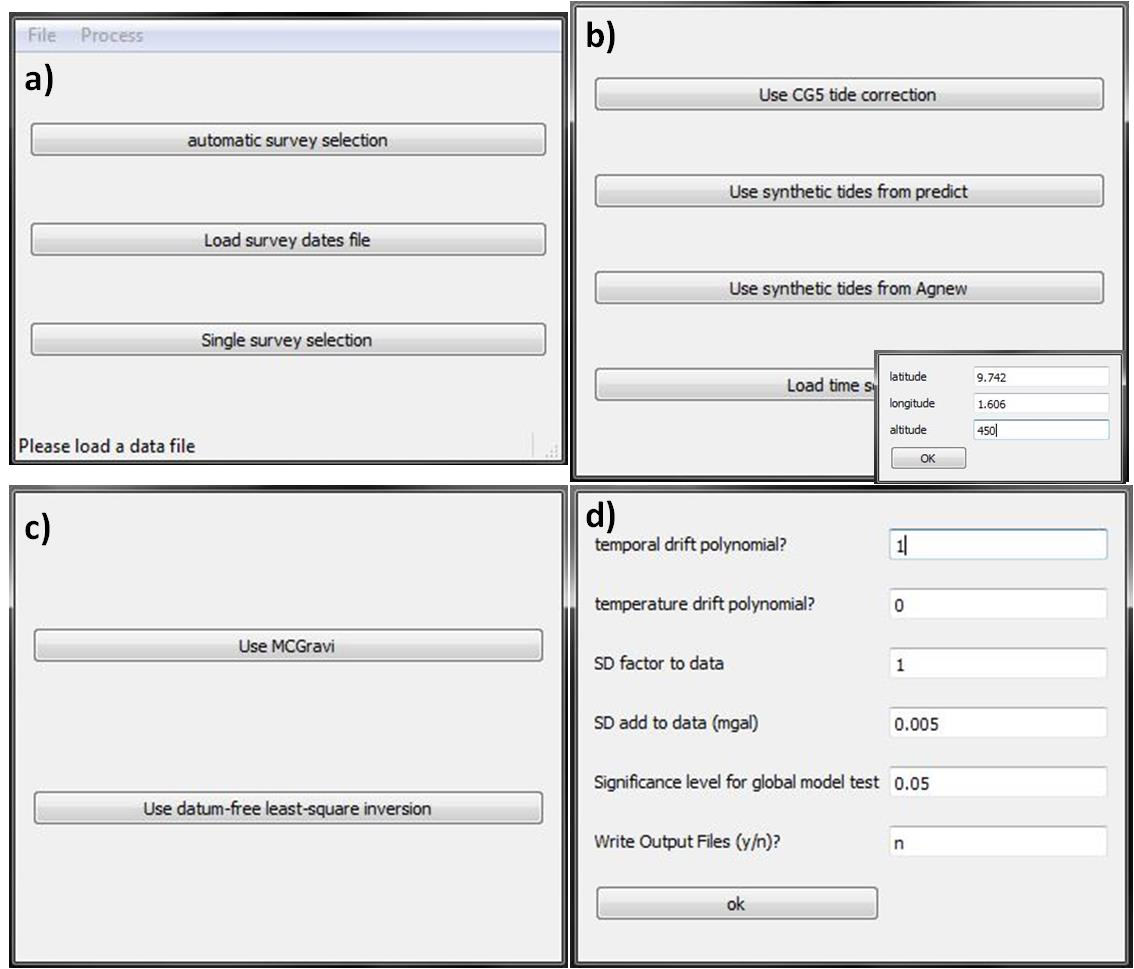
\includegraphics[width=\textwidth]{figures/example_of_pygrav_snapshots}
    \caption{Пример снимков \pg{}: a) Экран загрузки данных, b) Экран поправок
    за прилив, c) Экран компенсации сети и d) параметры компенсации сети.}
    \label{fig:example_of_pygrav_snapshots}
\end{figure}

\section[Загрузка данных]{Загрузка данных}
\label{sec:loading_data}

Доступны два варианта. Для продолжения/изменения обработки данных можно
загрузить <<raw data>> или <<processed data>>. При выборе <<processed data>>,
данные уже отсортированы в соответствии с иерархией съёмка/петля/пункты, в то
время как для <<raw data>> должны быть отсортированы. Таким образом, этот шаг не
только загружает данные, но и сохраняет их в соответствии с их иерархией (съёмки
-- петли -- пункты).

\subsection[Загрузка необработанных данных]{Загрузка необработанных данных}
\label{subsec:loading_raw_data}

Для выбора необработанных данных доступно три варианта:
\begin{itemize}
    \item Автоматический выбор съемки: для простой геометрии съемки, когда
    базовая станция всегда одна и та же, эта опция позволяет автоматически
    определять различные съемки на основе простого временного порога,
    запрошенного программой: выделяются разные съемки, если время между двумя
    последовательными сменами станций превышает пороговое значение. Если базовая
    станция и станция петли -- одни и те же, но имеют разные названия,
    следует выбрать параметр 0.

    \item Загрузка из файла даты начала/окончания съемки: эта опция позволяет
    считывать только съемки, определенные между датами начала и окончания,
    указанными во входном файле. Формат такого входного файла следующий:

    \begin{verbatim}
2012/07/11 05:17:00 2012/07/11 13:00:00
2012/07/13 05:00:00 2012/07/13 22:00:00
...
    \end{verbatim}
    
    \item Ручной ввод дату начала/окончания одной съемки (выбор единичной 
    съёмки)
    
\end{itemize}

Затем, петли в съёмках идентифицируются следующим образом: каждый раз,
когда обнаруживается базовая станция, запускается новый цикл, а предыдущий
завершается. Однако в более поздней процедуре корректировки дрейфа
обрабатываются вложенные петли, поскольку каждый цикл является частью одной и
той же системы уравнений, которая инвертируется с использованием метода
наименьших квадратов.

\subsection[Загрузка обработанных данных]{Загрузка обработанных данных}
\label{subsec:loading_processed_data}

Загрузка обработанных данных эквивалентна загрузке <<project>>. Она позволяет
повторно загрузить уже обработанные данные, которые должны быть предварительно
сохранены с помощью <<Save processed data>> (что эквивалентно сохранению
<<project>>), или упорядочены требуемым образом. Пользователю предлагается
загрузить файл, описывающий иерархию данных. Формат такого файла следующий:

\begin{verbatim}
Directory C:/Users/.../test_case/output_data/
Survey: 2013-09-19 nloops: 4 directory: 2013-09-19
Loop: 1 filename: fn111c13.262.txt
Loop: 2 filename: fn211c13.262.txt
Survey: 2013-09-21 nloops: 4 directory: 2013-09-21
Loop: 1 filename: fn111c13.264.txt
Loop: 2 filename: fn211c13.264.txt
Loop: 3 filename: fn311c13.264.txt
Survey: ...
Loop: ...
\end{verbatim}

Строки <<Survey>> описывают доступные съёмки, названия съёмок (дата первого
измерения), количество петель в съёмках, и названия папок
съёмок в корневом каталоге. Строки <<Loop>> описывают для каждой строки в каждой
съёмке название петли и файл данных петли. Файлы данных похожи на файлы CGxTool
'c', но без заголовка и дополнительного столбца, содержащего статус данных (1
или 0, независимо от того, сохранена строка данных для корректировки дрейфа или
нет).

\section[Поправки данных]{Поправки данных}
\label{sec:data_corrections}

\subsection[Земные приливы]{Земные приливы}
\label{subsec:earth_tides}

Доступны четыре варианта поправок за приливы:
\begin{itemize}
    \item Использование приливной поправки CG5 (ничего делать не нужно): до
    начала съемки в прибор должны быть введены географические координаты.

    \item Использование синтетических приливов из прогноза: для пользователей
    Window для создания синтетического прилива на основе приливных параметров,
    используемых для поправок, к программе подключается функция PREDICT из
    программного пакета ETERNA \cite{wenzel_1996} (см. раздел 8 об установке).
    В \pg{} запрограммирован приливной потенциала HW95 \cite{hartmann_hw95_1995},
    но при необходимости его легко изменить. Приливные параметры~-- это либо
    стандартные приливные параметры, либо вводимые пользователем в виде отдельного
    файла. Необходимо ввести географические координаты съемки.
    \begin{itemize}
        \item Экземпляр прогнозной программы (\verb|.exe|) должен быть доступен
        в папке с исходным кодом и копируется \pg{} в выходную папку, где
        производится вычисление.

        \item Стандартные приливные параметры считываются из файла (\verb|200D.INI|) в
        папке основного кода

        \item Формат файла приливных параметров, вводимых пользователем, должен
        быть следующим:

        \begin{verbatim}
0.023812    0.044652    1.13344    0.5445 MM
0.060132    0.080797    1.12607    -0.1195 MF
0.096423    0.249951    1.14548    0.6833 MTM
...
        \end{verbatim}
        (частота начала полосы пропускания (cpd) -- частота конца полосы пропускания (cpd) --
        амплитуда –- фаза –- название прилива)
        
    \end{itemize}

    \item Использование синтетических приливов из Agnew: это негармонический
    метод, предусмотренный кодами Fortran \cite{agnew_2007, agnew_2012}, и позже
    переведен в MATLAB\texttrademark{} \cite{cattin_gravprocess_2015} в
    программе \textbf{\textsf{GravProcess}}. В данном случае поправка
    представляет собой прямое вычисление приливного потенциала по
    \cite{munk_tidal_1966}. Он основан на внутренних эфемеридах (для определения
    положения Луны и Солнца). Необходимо указать местоположение съемки.

    \item Загрузка временных рядов: если в качестве временных рядов доступен
    другой синтетический прилив, его можно загрузить и использовать для  
    вычисления поправок. Принятый формат файлов~-- файлы \textbf{ETERNA} или
    \textbf{Tsoft} (\verb|.TSF|). Если расширение файла не \verb|.tsf|, он будет
    рассматриваться как внешний файл. По умолчанию данные должны храниться в
    первом канале (столбце).
    
\end{itemize}

\subsection[Океаническая нагрузка]{Океаническая нагрузка}
\label{subsec:ocean_loading}

Загрузку океана можно скорректировать, используя два различных подхода:
\begin{itemize}
    \item Если анализ приливов может быть выполнен на съёмочном пункте
    (например, благодаря близкому расположению сверхпроводящего гравиметра),
    можно перейти к поправке земных приливов, используя
    \textbf{\textsf{PREDICT}} из пакета \textbf{\textsf{ETERNA}} (см. выше) и
    предоставляя приливные параметры из анализа приливов. Этот эмпирический
    подход учитывает как земные приливы, так и поправку океанической нагрузки
    (но может также учитывать другие воздействия окружающей среды, такие как
    давление воздуха, которые происходят с аналогичной частотой).
    
    \item Коррекция океанической нагрузки в программе \pg{} такая же, как и в
    коде процесса \textbf{\textsf{Grave}} \cite{cattin_gravprocess_2015}. Он
    основан на \cite{agnew_2012} и на транскрипции MATLAB\texttrademark{} от
    \cite{cattin_gravprocess_2015}. Коэффициенты океанической нагрузки должны
    быть загружены из отформатированного файла, предоставленного свободным
    океаническим поставщиком Scherneck
    (\url{http://holt.oso.chalmers.se/loading/}). Параметры требуются для
    полусуточных (M2, S2, N2, K2), суточных (O1, P1, Q1, K1) и
    долгопериодических (MF, Mm, Ssa) приливных гармоник.
\end{itemize}

\subsection[Атмосфера]{Атмосфера}
\label{subsec:atmosphere}

Загрузите один временной ряд. Принятый формат файлов -- файлы
\textbf{\textsf{ETERNAL}} или \textbf{\textsf{Tsoft}} (\verb|.TSF|). Если
расширение файла не \verb|.tsf|, он будет рассматриваться как внешний файл. По
умолчанию данные должны храниться в первом канале (столбце).

\section[Выбор данных]{Выбор данных}
\label{sec:data_selection}

Это оригинальная функция программы. Иерархия данных видна в виде дерева, таблицы
и графического представления. Съемку, циклы, пункты и единичные измерения можно
проверить или снять флажок, следует ли их сохранять для процесса корректировки
дрейфа (и окончательных расчетов единичных разности). Это можно сделать либо
вручную, либо следуя автоматическим процедурам отбора, основанным на простых
пороговых критериях. В настоящее время к ним относятся 
\begin{itemize}
    \item пороговое значение для наклонов: не отмечаются абсолютные значения
    наклонов, превышающие входное значение
    
    \item пороговое значение стандартного отклонения силы тяжести (SD): не
    отмечаются значения SD, превышающие входные значения

    \item пороговое значение, основанное на значениях силы тяжести: не отмечаются значения
    абсолютной силы тяжести, превышающие среднее значение трех последних
    значений + входное пороговое значение

    \item критерий длительности: если длительность данных отличается от входного
    значения, они не отмечаются. Это часто происходит, когда пользователь
    сохраняет текущие данные в поле при остановке сбора CG5.

\end{itemize}

Когда выбраны отдельные пороговые значения, они применяются только к текущей
таблице. При нажатии кнопки \textbf{<<apply to all data>>} используются все
входные пороговые значения, причем для всего набора данных.

Другой вариант быстрой проверки/снятия флажков с данных -- выделить несколько
строк с помощью мыши и нажать кнопки \textbf{<<check selected>>} или
\textbf{<<uncheck selected>>}.

Каждая съёмка и петли идентифицируются по датам их первых измерений.
Указаны номера станций, а число в скобках -- это номер повторения, поскольку
некоторые станции повторяются (например, базовая станция). Данные организованы в
хронологическом порядке.

Ручной выбор может быть выполнен на основе табличных значений или графических
отображений, в зависимости от предпочтений пользователя. На графическом дисплее
непроверенные данные отображаются черным цветом, в то время как отмеченные
данные -- синим. На экране значения силы тяжести, среднее значение выбранных данных
отображается синей горизонтальной линией.

После выбора данных следует нажать кнопку OK. Это действие мало что дает, но
может быть важным: оно используется для проверки того, что на некоторых пунктах 
данные не выбраны, и в этом случае они удаляются. Это может произойти с помощью
автоматического выбора.

\section[Уравнивание дрейфа]{Уравнивание дрейфа}
\label{sec:drift_adjustment}

Как только поправки будут применены и данные выбраны, можно приступать к
корректировке дрейфа. Доступны два варианта. Можно запустить либо
\textbf{\textsf{MCGravi}} \cite{beilin_2006} (если он установлен, см.
раздел~\ref{chap:installing_external_programs}), либо использовать простую схему
инверсии наименьших квадратов без данных \cite{hwang_adjustment_2002}.
Единственный интерес в использовании \textbf{\textsf{MCGravi}} заключается в
том, что выполняется компенсация сети и необходимо использовать несколько
фиксированных абсолютных (априорных) значений (используя опцию
\textbf{<<weighted constraint>>}). Для этого требуется чтобы была доступна
\verb|mcgravi.exe|. Программа записывает входные файлы \textbf{\textsf{MCGravi}}
в выходной каталог и считывает выходные файлы \textbf{\textsf{MCGravi}} (файл
\verb|*.gra| в папках mix\dots). 

Пользователь может выбрать параметры для применения к данным перед инверсией:
\begin{itemize}
    \item Коэффициент SD: мультипликативный коэффициент на наблюдаемое
    стандартное отклонение (SD)
    
    \item SD\_add: константа, добавляемая к каждому наблюдаемому SD
\end{itemize}

Также следует указать время и температурный дрейф в градусах.

Единичные разности отображаются в консоли и могут быть сохранены в виде файла
\verb|SimpleDifferences.dat| в каждой папке опроса выходного каталога, выбрав
\textbf{File} $\rightarrow$ \textbf{Save simple differences}.

\section[Вычисление двойных разностей]{Вычисление двойных разностей}
\label{sec:compute_double_differences}

Как только вычислены единичные разности, двойные разности могут быть вычислены с
помощью \textbf{Process} $\rightarrow$ \textbf{Compute double differences}.
Затем двойные разности можно сохранить в выходной папке, выбрав \textbf{File}
$\rightarrow$ \textbf{Save double difference}. Это создаст файлы двойных
разностей силы тяжести и SD в выходном каталоге. Доступны два формата (даты --
пункты или пункты -- даты).
\chapter[Пример для проверки]{Пример для проверки}
\label{chap:test-case}

В этом разделе подробно описаны два способа обработки тестового примера. Первый
использует графический интерфейс \pg{} для быстрой и удобной обработки данных
микрогравиметрии. Второй использует сценарий Python, который вызывает функции
\pg{}. Это больше всего подходит для тех, кто заинтересован в разработке \pg{} и
добавлении новых функциональных возможностей.

\section[Использование графического интерфейса pyGrav]{Использование графического интерфейса pyGrav}
\label{sec:using_pygrav_gui}

Тестовый пример доступен в каталоге \verb|test_case|. Это набор из 4 съемок,
проведенных в ходе Западноафриканской кампании в небольшом водосборном бассейне
на севере Бенина. Каждая съемка обычно состоит из четырех петель, охватывающих в
общей сложности 13 пунктов и базовую станцию (станция \textnumero{}~1). 

Чтобы обработать этот набор данных из файла необработанных данных, выполните
следующие действия:
\begin{itemize}
    \item Запустите \pg{}: запустите файл Python \verb|pyGrav_main.py| используя
    python(x,y), например, в Windows, или выполнив \verb|python pyGrav_main.py| в
    оболочке Linux.

    \item Запустите проект: выберите подкаталоги \verb|input_data/raw| и \verb|output_data| из
    каталога \verb|test_case|.

    \item Выберите \textbf{Load raw data} в меню \textbf{File}: откройте \verb|Atest_Raw_data.txt|

    \item Выберите \textbf{Load Survey dates file} и загрузите
    \verb|Atest_start_end_dates.txt|, или в качестве альтернативы, выберите одну
    съёмку путём введения начальных и конечных дат (см. файл
    \verb|Atest_start_end_dates.txt|). Номер базовой станции равен 1.

    \item Обработка приливов: Выберите \textbf{Tide corrections} в меню
    \textbf{Process} и выберите \textbf{Use CG5 tide corrections} или в качестве
    альтернативы \textbf{Use Synthetic tides from predict} (если установлено,
    см. раздел~\ref{chap:installing_external_programs}): Широта = 9.742; Долгота
    = 1.606; Высота над уровнем моря = 450. В этом случае выберите \textbf{Load
    Tidal parameters} и загрузите \verb|tide_param.txt| из папки
    \verb|input_data|. Этот список параметров был получен на основе приливного
    анализа сверхпроводящего гравиметра, доступного на месте исследования, и
    следовательно, эмпирически включает океаническую нагрузку.  В качестве
    последнего варианта, выберите \textbf{Use Synthetic tides from Agnew}:
    Широта = 9.742; Долгота = 1.606; Высота над уровнем моря = 450.

    \item Обработка океанической нагрузки: выберите \textbf{Ocean Loading correction} в
    меню \textbf{Process} и выберите файл \verb|oceantidal.txt| из папки \verb|input_data|. Этот файл
    был получен из \url{http://holt.oso.chalmers.se/loading/} с широтой = 9.742;
    долготой = 1.606; высотой над уровнем моря = 450.

    \item Выбор данных: выберите \textbf{Data selection} в меню \textbf{Process}.
    \begin{itemize}
        \item Перейдите в дерево на левой панели, чтобы проверить временные ряды
        для некоторых пунктах, щелкнув на пункт в петле. Сначала все измерения
        проверяются и отображаются синим цветом в окнах графика (правая панель).
        
        \item Попробуйте снять галочки с некоторых данных в табличном
        представлении. Графики обновляются при повторном нажатии на пункт в
        дереве (левая панель) или при нажатии кнопки \textbf{update plots} на верхней
        панели. Черные точки появляются там, где данные не отмечены. Эти
        измерения не будут сохранены для компенсации сети. Горизонтальная синяя
        линия на графике силы тяжести -- это среднее значение силы тяжести для
        отмеченных значений.

        \item Автоматический выбор. Заполните следующие критерии автоматического
        выбора и выберите \textbf{apply to all data}:
        \begin{itemize}
            \item \textbf{auto uncheck tilts >}: 5
            \item \textbf{auto uncheck g >}: 4
            \item \textbf{auto uncheck SD >}: 20
            \item \textbf{auto uncheck dur <>}: 60
        \end{itemize}

        \item Просмотрите подборку, чтобы завершить фактический выбор (при
        необходимости).

        \item Нажмите кнопку OK. Это действие мало что дает, но может быть
        важным: оно используется для проверки того, что на некоторых станциях
        данные не выбраны, и в этом случае они удаляются. Это может произойти с
        помощью автоматического выбора.
        
    \end{itemize}
    
    \item Теперь обработанные данные можно сохранить: в меню \textbf{File}
    выберите \textbf{Save processed data}. В папке \verb|output_data| будут
    созданы подкаталоги, имена которых являются именами съёмок и которые
    содержат файлы петель, аналогичные файлам CGxTool 'c', с дополнительным
    столбцом 0 или 1, указывающим, следует ли сохранить станцию или нет. Вся
    иерархия данных записана в файле \verb|gravity_data_hierarchy.txt| в папке
    \verb|output_data|. Этот файл можно открыть в другом проекте для загрузки
    обработанного набора данных (выбрав пункт загрузить обработанные данные в
    меню Файл).
    
    \item Коррекция дрейфа: выберите \textbf{Drift Adjustment} в меню
    \textbf{Process} и \textbf{Use datum-free least-square inversion} без
    привязки к данным с параметрами:
    \begin{itemize}
        \item \textbf{Temporal drift polynomial?}: 1
        \item \textbf{Temperature drift polynomial?}: 0
        \item \textbf{SD factor to data}: 1
        \item \textbf{SD add to data (mgal)}: 0.005
        \item \textbf{Significance level for global model test}: 0.05 (т.~е. 5\%)
        \item \textbf{Write Output Files (y/n)?}: y
    \end{itemize}

    \item Теперь дрейф скорректирован и можно проверить выходные файлы, чтобы
    увидеть, удовлетворяет ли вывод дрейфа или нет. В каждой подпапке съёмки 
    (которая была создана, если она ранее не была создана функцией \textbf{Save
    processed data}) из папки \verb|output-data| два файла, начинающихся с
    \verb|LSresults|, отображают результаты единичных разностей для первого и полную
    процедуру LS (ввод, выходные данные и полная проверка) для второго.

    \item Сохранение единичных разностей: выберите \textbf{Save simple difference} в меню
    \textbf{File}. Как и в случае с функцией \textbf{Save processed data}, это создаст
    файлы единичных разностей во вложенных папках папки \verb|output_data| вместе с файлом
    иерархии, начинающимся с \verb|simple_diff_data_hierarchy...txt|

    \item Вычисление двойной разности: выберите \textbf{Compute double difference} в меню
    \textbf{Process}. Выберите опорную съёмку, например, первую. Затем выберите
    \textbf{Classic double difference}.

    \item Теперь возможно сохранить двойные разности: выберите \textbf{Save
    double difference} в меню \textbf{File}. Это создаст файлы \verb|gravity| и
    \verb|SD double difference| в каталоге \verb|output_data|. Доступны два
    формата (даты -- пункты или пункты -- даты).

    \item Альтернативой здесь является загрузка уже обработанных данных (в
    данном случае, уже выбранных данных), и для сравнения результатов
    уравниваний дрейфа, единичных и двойных разностей с выбранными вами
    результатами. В этом случае начните с изменения пути к данным в первой
    строке файла \verb|gravity_data_hierarchy.txt| в каталоге
    \verb|input_data/preprocessed|. Затем выберите пункт \textbf{Load processed
    data} в меню \textbf{File} и выберите файл \verb|gravity_data_hierarchy.txt| в
    каталоге \verb|input_data/preprocessed|. Этот файл является файлом иерархии,
    описывающим, где найти файлы петли в каждом каталоге съёмки (как указано в
    функции \textbf{Save processed data}).
    
\end{itemize}

\section[Использование сценариев python и объектов pyGrav]{Использование сценариев python и объектов pyGrav}
\label{sec:using_a_python_script_and_pygrav_objects}

Другой способ использования функций \pg{} (в \verb|data_objects.py| файл)
заключается в написании сценария на Python и последовательном вызове этих
функций. Это особенно подходит, если кто-то хочет добавить функцию в основной
код и протестировать ее, не проходя через все программирование с графическим
интерфейсом. Как только функция настроена должным образом, дополнительные
кнопки/действия графического интерфейса могут быть легко добавлены в
\verb|pyGrav_main.py| путем адаптации существующего кода.

Пример сценария (\verb|example_script.py|) можно найти в каталоге
\verb|main_code|, и он должен выполняться как скрипт на Python. Цель скрипта --
загрузить необработанные данные, извлечь отдельные съёмки на основе дат начала и
окончания, выбрать данные для сохранения на основе простых пороговых значений,
уравнять дрейф для каждой съёмки, и в конечном итоге вычислить как единичные,
так и двойные разности. Комментируя/раскомментируя некоторые части кода, также
можно загрузить уже выбранные и упорядоченные данные.
\chapter[Структура кода]{Структура кода}
\label{chap:code_structure}

\section[Объектно-ориентированное программирование и данные микрогравиметрии]{Объектно-ориентированное программирование и данные микрогравиметрии}
\label{sec:object-oriented programming_and_microgravity_data}

Этот мощный способ программирования, для которого особенно подходит Python,
основан на наборе определений объектов (классов), которые содержат оба атрибута
(или свойства), такие как временной ряд, имя, словарь других объектов… и методы
(или функции/определения), которые описывают, что может делать объект. Таким
образом, этот метод программирования не является линейным, но способствует
удобочитаемости кода, как только программист привыкает к таким концепциям.
Метод, например, для записи новых выходных форматов, может быть легко добавлен в
соответствующий объект и вызван из основной программы, добавив всего несколько
строк и сохранив общий фрейм исходного кода.

Это особенно подходит для данных о микрогравитации, главным образом потому, что
данные могут быть организованы в виде структур (объектов) в соответствии с
иерархическим определением (кампания, которая включает в себя несколько опросов,
которые включают в себя несколько циклов, которые включают в себя несколько
станций, которые включают временные ряды полученных данных). Объекты могут быть
физически идентифицированы (кампания, опрос, цикл, станция), а также связанные с
ними методы (чтение ascii-файла CG5 должно быть определено в самом широком
объекте - кампании; запись входного файла mcgravi – файла ‘c’ - для
корректировки дрейфа должна быть определена в объекте цикла, в то время как
корректировка дрейфа должна вызываться или основываться на объекте съемки; выбор
данных будет в основном касаться станций). Эта логическая иерархия позволяет
хранить данные в виде структур.

\section[Графический интерфейс и PyQt]{Графический интерфейс и PyQt}
\label{sec:gui_and_pyqt}

yQt использует мощный язык программирования python и его пригодность для
объектно-ориентированного программирования вместе с библиотеками Qt GUI
(графический пользовательский интерфейс). PyQt состоит из нескольких модулей,
таких как фундаментальный QtCore (для функций, отличных от gui, таких как
использование файлов, потоков, процессов или времени) и QtGui (для графических
компонентов), среди которых определены от десятков до сотен классов, содержащих
многочисленные функции и свойства.

\section[Код pyGrav]{Код pyGrav}
\label{sec:pygrav_code}

Код основан на объектно-ориентированном программировании (ООП). Это можно
рассматривать как два параллельных набора определений:
\begin{itemize}
    \item Функции хранения данных и манипулирования ими: ядро программы, где
    определены классы и функции для операций с данными. Это тот самый
    \verb|data_object.py| исходный файл.

    \item Функции GUI: функции графического интерфейса пользователя, которые
    связывают требования пользователя с операциями с данными, определенными в
    предыдущем наборе определений. Это тот самый \verb|pyGrav_main.py| исходный
    файл.
    
\end{itemize}

В целом, код обильно прокомментирован, и описан каждый класс, подкласс, функции и свойства.

\subsection[Объектный файл данных]{Объектный файл данных}
\label{subsec:data_object_file}

Этот модуль содержит основные классы программы:
\begin{itemize}
    \item Базовый класс - это объект типа Channel List, который в основном
    содержит списки каналов, подобные тем, что содержатся в выходных файлах CG5
    ascii (сила тяжести, наклоны, температура, стандартное отклонение, время
    ...).

    Производные классы следуют логической иерархии, где каждый "подкласс"
    создается как элемент словаря из родительского класса:
    \begin{itemize}
        \item класс Campaign содержит словарь объектов типа "Опрос"
        \begin{itemize}
            \item class Survey содержит словарь объектов типа "Цикл".
            % \begin{itemize}
                \item цикл класса содержит словарь объектов типа 'Station'.
                % \begin{itemize}
                    \item станция класса o содержит временные ряды для каждой станции
                % \end{itemize}
            % \end{itemize}
        \end{itemize}
    \end{itemize}
    
\end{itemize}

Каждый из этих объектов является производным от объекта списка каналов.
Экземпляр базового класса 'Campaign' содержит весь набор данных. У каждого
класса также есть определенные свойства и функции заполнения, записи, обработки
и processing, вызываемые из основной программы (рис. 1).

\begin{figure}
    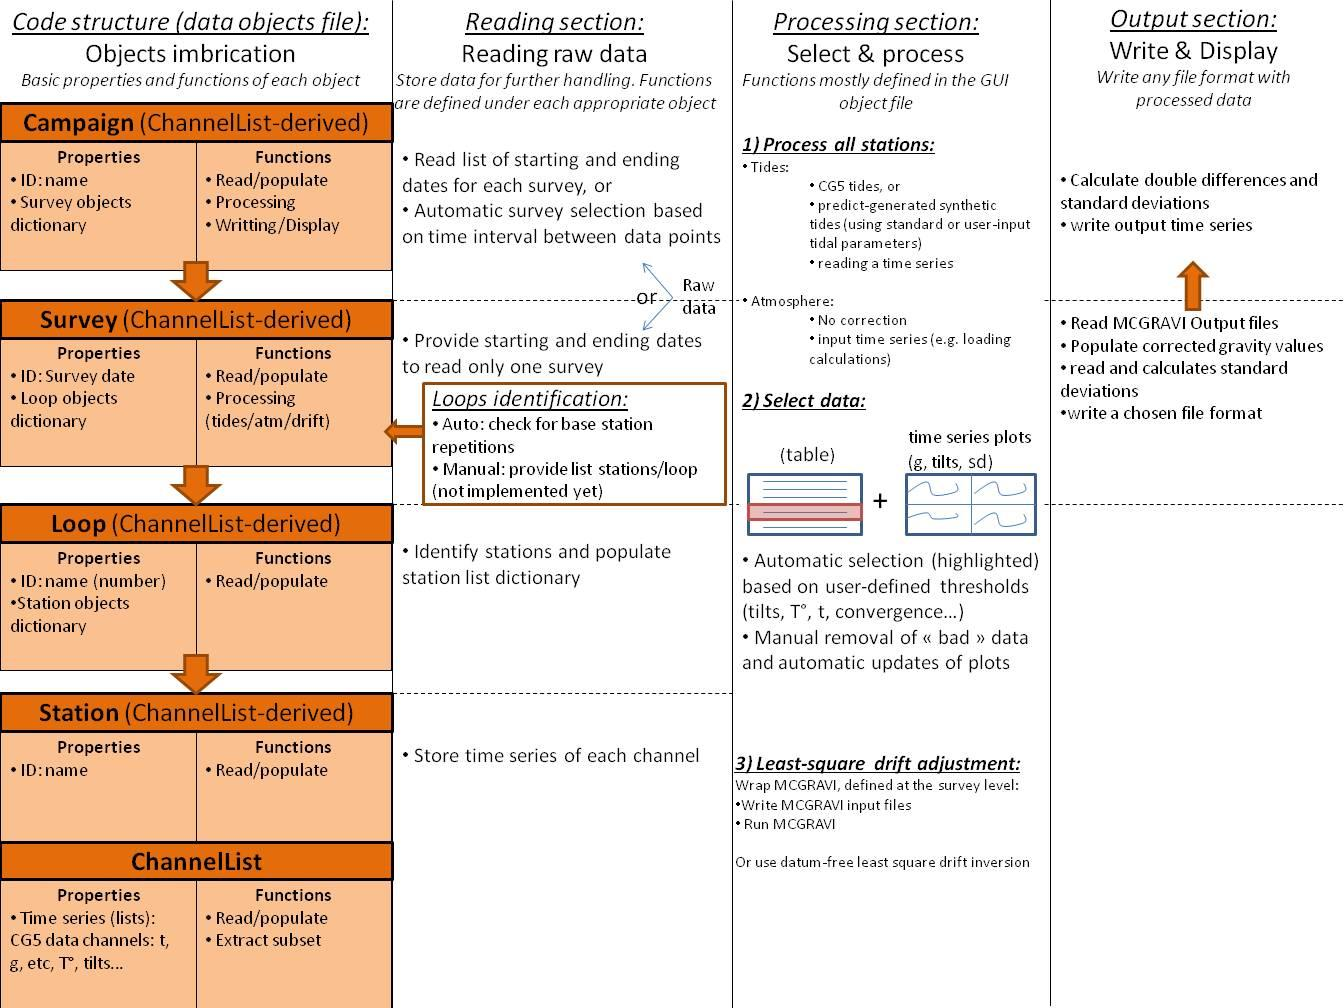
\includegraphics[width=\textwidth]{figures/pygrav_chart_and_structures_imbrications}
    \caption{Диаграмма pyGrav и обозначения структур (объектов) : в объекте
    кампании есть словарь из нескольких опросов. В объекте обзора есть словарь
    из нескольких циклов. В объекте цикла есть словарь из нескольких станций.
    Каждый из этих объектов является производным от объекта Channel List (т.е.
    они содержат несколько временных рядов).}
    \label{fig:pygrav_chart_and_structures_imbrications}
\end{figure}

\subsection[Файл графического интерфейса]{Файл графического интерфейса}
\label{subsec:gui_file}

Это файл, который должен быть выполнен для запуска pyGrav. Он содержит
единственный класс под названием main Prog, который является объектом
QMainWindow, производным от Qt. Наиболее важными свойствами класса mainProg
являются объект Campaign, который содержит весь набор данных, а также каталоги
данных и выходных данных. Большинство функций класса mainProg связывают
пользовательский интерфейс (определенный в функциях) с кодом обработки,
записанным в файле объекта данных, для изменения состояний объекта Campaign
(набора данных).

\section*{Ссылки}

Несколько ссылок для тех, кто заинтересован в изменении кода

Несколько руководств по Python:

\url{https://docs.python.org/2/tutorial/} Руководство для Python версии 2.7

\url{http://zetcode.com/lang/python/}

\url{http://marvin.cs.uidaho.edu/Teaching/CS515/pythonTutorial.pdf} (Руководство G. Van Rossum)

Руководство PyQt:

\url{http://zetcode.com/gui/pyqt4/}

Ссылки на класс PyQt:

\url{http://pyqt.sourceforge.net/Docs/PyQt4/classes.html}

Демо графиков PyQt:

\url{http://eli.thegreenplace.net/2009/05/23/more-pyqt-plotting-demos/}

Руководства программирования вида модели:

\url{http://www.yasinuludag.com/blog/?p=98}

Руководство Matplotlib:

\url{http://web.archive.org/web/20100830233506/http://matplotlib.sourceforge.net/leftwich_tut.txt}
\chapter[Протокол получения данных]{Протокол получения данных}
\label{chap:acquisition_protocol}

Для правильной работы программы требуются некоторые основные шаги, касающиеся
процедуры сбора данных. Некоторые процедуры сбора данных также следует применять
в более общем смысле, чтобы получать более точные результаты и проводить
эффективные обследования. Подробный анализ и описание гравитационных сетей см.,
например (\cite{lambert_nano_1977, torge_1980}). Требования и рекомендации по
высококачественным проектам обследования можно найти в \cite{seigel_1995}.

\section[Геометрия петли и номенклатура]{Геометрия петли и номенклатура}
\label{sec:loop_geometries_and_nomenclature}

\begin{itemize}
    \item Отдельные пункты всегда должны иметь один и тот же идентификационный
    номер (название), независимо от их статуса (опорный/рядовой
    пункт). Если он изменен, его можно модифицировать вручную, используя процедуру
    поиска/замены в файле необработанных данных в текстовом редакторе.
    
    \item Различные опорные пункты в рамках одной схемы обработки до сих пор не
    обрабатываются, но программа может запускаться последовательно для каждого
    подмножества данных.
    
    \item Предпочтительно, но не обязательно, чтобы опорный пункт имел другое
    название, чем пункт цикла (если он соответствует тому же местоположению).
    
\end{itemize}

\section[Транспортировка]{Транспортировка}
\label{sec:transportation}

\begin{itemize}
    \item CG5 очень чувствителен к транспортировке: на короткие расстояния его
    могут переносить два оператора, которые держат рейку, на которую за ручки
    подвешен мешок с гравиметром. На больших расстояниях он должен быть в лучшем
    случае изолирован от вибрации автомобиля.

    \item Транспортировка обычно подразумевает так называемый кратковременный
    "транспортный дрейф", и стабилизация пружины после достижения станции может
    занять некоторое время. Этап выбора данных в pyGrav позволяет выбрать данные
    после стабилизации прибора.

\end{itemize}

\section[Настройка прибора]{Настройка прибора}
\label{sec:setting_up_the_instrument}

\begin{itemize}
    \item Поскольку вертикальные перемещения сильно влияют на изменение силы
    тяжести ($\approx$0,3 мкгал/мм при номинальном градиенте свободного воздуха),
    станции должны быть оборудованы бетонными опорами, чтобы ограничить
    последствия мягкого грунта или других неустойчивых элементов.В качестве
    альтернативы можно было бы использовать приводные стержни для ограничения
    роли усадки/набухания грунта. Для каждой съемки (в режиме замедленной
    съемки) прибор должен располагаться точно в одной и той же точке и
    удерживаться под одним и тем же азимутом, например, благодаря винтам,
    воткнутым в бетонную стойку. Высоту относительно стойки следует поддерживать
    постоянной с помощью латунного кольца, прикрепленного к одной ножке штатива
    прибора, как предложил \cite{montgomery_1971}.
    
    \item CG5 и его штатив должны быть защищены от ветра и прямых солнечных
    лучей, например, мусорным баком, покрытым изоляционным материалом, или
    соответствующим зонтиком.
    
\end{itemize}

\section[Сбор данных]{Сбор данных}
\label{sec:data_acquisition}

\begin{itemize}
    \item В настоящее время нет возможности применить различные поправки к
    приливам в рамках одной и той же съемки. Следовательно, если съемка состоит
    из станций, удаленных друг от друга на большое расстояние (несколько
    десятков км, не рекомендуется для высокоточных покадровых гравитационных
    съемок), пользователь должен позаботиться о том, чтобы ввести правильные
    местоположения станций в CG5 на местах, чтобы можно было применить поправку
    CG5 на земные приливы.
    
    \item Длительность: CG5 производит выборку с частотой 6 Гц и усреднение по
    заданной пользователем длительности для получения одного единственного
    измерения. \cite{merlet_micro-gravity_2008} показали в своем исследовании, что
    отклонение по Аллану их CG5 достигло 1 мкгал через 40 с, до минимума в 0,8
    мкгал через 85 с, но еще больше увеличилось из-за влияния приливов.
    \cite{gettings_techniques_2008} также показывают пример из необработанных
    данных за 1 секунду (их рисунок 2), где среднее значение сходится примерно
    через 40 секунд.  Кроме того, по истечении 60 секунд стандартная ошибка на
    экране дисплея CG5, работающего в полевых условиях, всегда, по-видимому,
    сходится. Хранение данных за 60 секунд часто позволяет сделать динамичный и
    быстрый вывод о стабильности прибора (см., например, \cite{hector_water_2015}).

    \item Идентификация стабилизации: Существует столько вариантов, сколько
    требуется пользователям и научным целям для определения того, является ли
    полученный временной ряд достаточно длинным (стабилизированным) или нет.
    Строгая процедура идентификации сигналов малой амплитуды при покадровых
    исследованиях может быть следующей: на станции проводится первая серия из 5
    измерений, пока операторы находятся на расстоянии нескольких метров от
    прибора, прежде чем в первый раз проверяется выравнивание. Затем проводится
    еще один набор измерений, и операторы приходят проверять стабильность работы
    прибора примерно каждые 5 минут. При любой проверке, если наклоны выходят за
    пределы диапазона 0 ± 5 дюймов (или любого другого выбранного порогового
    значения), прибор снова выравнивается. Это следует за \cite{merlet_micro-gravity_2008},
    которые обнаружили, что внутренняя коррекция наклона CG5 является точной на
    уровне 1 мкгал при ± 20‘. Кроме того, им удалось сохранить наклоны в
    пределах 0 ± 3 ’ в условиях их внутреннего и стабильного пирса. Измерения
    можно считать выполненными (и гравиметр стабильным), если выполнены все
    следующие критерии: - выполнено минимум 10 соответствующих измерений; -
    изменения силы тяжести составляют 3 мкгал или менее в течение 5
    последовательных измерений; - в 5 последних измерениях нет видимого дрейфа
    (дрейф <1 мкгал/мн).. Все это означает, что долгосрочный дрейф CG5 внутренне
    корректируется прибором, скажем, при остаточном дрейфе < 100 мкгал/сут
    (около 1 мкгал/15млн).
    
\end{itemize}
\chapter[Среднеквадратическая инверсия и распределение ошибок]{Среднеквадратическая инверсия и распределение ошибок}
\label{chap:least-square_inversion_and_error_propagation}

Гравиметрические наблюдения на пункте представляют собой временные ряды из
нескольких измерений силы тяжести, каждое измерение является средним значением
нескольких выборок. Например, типичные результаты измерения CG-5 получены в
результате сбора фрагментов в течение более минуты (наилучшим считается 85
секунд \cite{merlet_micro-gravity_2008}) при частоте 6 Гц. Таким образом,
стандартная погрешность (SE) при каждом измерении составляет:
\begin{equation}
    SE = \frac{\sigma}{\sqrt{n}}
\end{equation}
где $\sigma$~-- стандартное отклонение измерения, а $n$~-- количество выборок.

После отбора данных из оставшихся временных рядов выводятся одно наблюдение $l_i$
и стандартное отклонение $\sigma_i$ для каждого пункта $i$ с использованием средних,
взвешенных по дисперсии:
\begin{equation}
    l_i = \frac{\sum_{j=1}^{n}\frac{1}{SE^2_j}}{\sum_{j=1}{n}\frac{1}{SE^2_j}}
\end{equation}
\begin{equation}
    \sigma_i = \frac{1}{\sum_{j=1}^{n}\frac{1}{SE_j^2}}
\end{equation}

Стандартное отклонение $\sigma_{ij}$ для наблюдения относительной силы тяжести
$\Delta l_{ij}$ между пунктами $i$ и $j$ определяется как
\begin{equation}
    \sigma_{ij} = \sqrt{\sigma_i^2 + \sigma_j^2},
\end{equation}
где $\Delta l_{ij}$ определяется как
\begin{equation}
    \Delta l_{ij} + \upsilon_{ij} = g_j + g_i + \sum_{T=1}^{m} a_T\left(t_j - t_i\right)^T + \sum_{k=1}^{m} b_k \left(t_j - t_i\right)^k
\end{equation}

Здесь $\upsilon_{ij}$~-- невязки, $g_i$~-- значение силы тяжести на пункте $i$,
$m$~-- степень полинома коэффициентов $a_T$ для дрейфа гравиметра и $n$~--
степень полинома коэффициентов $b_k$ для температурного дрейфа. Таким образом,
система уравнений является
\begin{equation}
    \mathbf{L}^{\mathbf{b}} + \mathbf{V} = \mathbf{A}\mathbf{X},
\end{equation}
где $\mathbf{L}^{\mathbf{b}}$ вектор, содержащий $n$ наблюдений относительной
силы тяжести, $\mathbf{V}$~-- вектор с $n$ невязками, $\mathbf{A}$~--
дизайн-матрица и $\mathbf{X}$~-- вектор $u$ неизвестных (значений силы тяжести и
параметров дрейфа). Чтобы получить решение $\mathbf{X}$, необходимо удерживать
фиксированным по крайней мере одно значение силы тяжести во время уравнивания
(так называемое исходное значение силы тяжести). Здесь это делается путем
добавления наблюдений абсолютного значения силы тяжести (обычно равной нулю) на
опорном пункте:
\begin{equation}
    \mathbf{L}^{\mathbf{b}}_{\mathbf{g}} + \mathbf{V}_{\mathbf{g}} =
    \mathbf{A}_{\mathbf{g}\mathbf{X}} =
    \left[\mathbf{I}0\right]
    \left[
        \begin{aligned}
            \mathbf{X}_{\mathbf{g}}\\
            \mathbf{X}_{\mathbf{I}}
        \end{aligned}
    \right]
\end{equation}

Введя вектор $S$ с $k$ (числом значений силы тяжести), первые значения которых равны
единице, а последние значения $u-k$ равны нулю, что удовлетворяет:
\begin{equation}
    \mathbf{S}^{\mathbf{T}}\mathbf{X}=0
\end{equation}
можно найти решение по методу наименьших квадратов для $X$:
\begin{equation}
    \mathbf{X} = \left(\mathbf{A}^{\mathbf{T}}\mathbf{P}\mathbf{A} + \mathbf{S}\mathbf{S}^{\mathbf{T}}\right)^{-1}\mathbf{A}^{\mathbf{T}}\mathbf{P}\mathbf{L}^{\mathbf{b}}
\end{equation}

Матрица весов $\mathbf{P}$ состоит из членов, обратных дисперсии для наблюдений.

Апостериорная дисперсия единичного веса ($\sigma^2_0$) задается формулой
\begin{equation}
    \sigma^2_0 = \frac{\mathbf{V}^{\mathbf{T}}\mathbf{P}\mathbf{V}}{n+1-u}
\end{equation}
и апостериорная ковариационная матрица $\mathbf{S}_X$ задается путем
распространения ковариации:
\begin{equation}
    \mathbf{S}_X = \sigma^2_0\left(\mathbf{A}^{\mathbf{T}}\mathbf{P}\mathbf{A}+\mathbf{S}\mathbf{S}^{\mathbf{T}}\right)^{-1}
    \mathbf{A}^{\mathbf{T}}\mathbf{P}\mathbf{A}\left(\mathbf{A}^{\mathbf{T}}\mathbf{P}\mathbf{A}+\mathbf{S}\mathbf{S}^{\mathbf{T}}\right)^{-1}
\end{equation}

Код также переходит к проверке по глобальной модели, чтобы оценить, адекватна
ли математическая модель или в данных есть отклонения. Если выполняется
следующее условие, то модель уравнивания можно считать правильной и
завершенной до уровня значимости $\alpha$:
\begin{equation}
    \chi^2=\frac{\mathbf{V}^{\mathbf{T}}\mathbf{P}\mathbf{V}}{\sigma^2_{0i}}<\chi^2_c\left(1-\alpha;m\right)
\end{equation}
где $\sigma^2_{0i}$ -- априорная дисперсия единичного веса, а
$\chi^2_c\left(1-\alpha;m\right)$ -- критическое значение распределения
$\chi^2$, когда доверительный уровень равен $\alpha$, а степень свободы уравнивания 
равна $m$.
\begin{equation}
    \chi^2_c\left(1-\alpha;m\right)=m\left[\chi_{1-\alpha}\left(\frac{2}{9m}\right)^{\frac{1}{2}}+1-\left(\frac{2}{9m}\right)\right]^3
\end{equation}
и для $0<\alpha<0.5$
\begin{equation}
    \chi_{1-\alpha} = t - \frac{2.515517 + 0.802853t + 0.010328t^2}{1 + 1.432788t + 0.189269t^2 + 0.001308t^3}
\end{equation}
и
\begin{equation}
    t = \sqrt{2\ln \left(\frac{1}{\alpha}\right)}
\end{equation}
\chapter[Установка сторонних программ]{Установка сторонних программ}
\label{chap:installing_external_programs}

pyGrav предоставляет фрейм для обработки данных о микрогравитации. Таким
образом, легко возможно включить вызовы внешних программ в pyGrav. В настоящее
время могут быть вызваны две программы: функция ПРОГНОЗИРОВАНИЯ из пакета ETERNA
\cite{wenzel_1996} для расчета синтетических приливов и MCGRAVI \cite{beilin_2006} для
настройки сети. Чтобы добавить любой другой вызов к внешним программам, лучший
способ~-- просмотреть скрипты pyGrav и вдохновиться тем, как эти две программы
взаимодействуют. Здесь описана установка таких программ, если они будут
использоваться в pyGrav

\section[Установка ETERNA]{Установка ETERNA}
\label{sec:eterna_installation}

Для пользователей window можно использовать функцию ETERNA из пакета ETERNA
\cite{wenzel_1996} для коррекции приливов. Это особенно подходит, когда доступны
параметры приливов для конкретного участка (например, с помощью анализа приливов
по данным сверхпроводящего гравиметра, поскольку это также включает эффект
океанической нагрузки). Каталог pyGrav включает в себя облегченную версию ETERNA
с минимумом, необходимым для правильной работы функции ПРОГНОЗИРОВАНИЯ. Просто
скопируйте папку /eterna33 из папки \verb|main_code/external_files/| в корневой каталог
(\verb|C:\|). Когда pyGrav попросят запустить \verb|predict|, он скопирует экземпляр
\verb|predict.exe| файл, присутствующий в папке \verb|main_code/external_files/|, в выходной
каталог опроса и запустите его. Это \verb|predict.exe| затем программа вызовет данные о
приливном потенциале из \verb|C:/eterna33| папка. Полный пакет услуг ETERNA также
доступен бесплатно в кассе: \url{http://www.upf.pf/ICET/soft/index.html}.

\section[Установка MCGRAVI]{Установка MCGRAVI}
\label{sec:mcgravi_installation}

MCGravi (Beilin, 2006) может использоваться для корректировки дрейфа по методу
наименьших квадратов и компенсации сети в случае сложной сети с несколькими
известными абсолютными точками (взвешенная инверсия наименьших квадратов
ограничения, см. \cite{hwang_adjustment_2002}). В качестве альтернативы,
алгоритм инверсии наименьших квадратов без данных \cite{hwang_adjustment_2002}
закодирован в pyGrav.

\begin{itemize}
    \item Скопируйте папку MCGRAVI в корневой каталог (\verb|C:\|) (или в другое место).

    \item МАКГРОУ, возможно, мне потребуется перекомпилировать. В этом случае
    необходим G95. Его можно найти здесь:
    \url{http://www.g95.org/downloads.shtml}, или
    \url{http://math.hawaii.edu/~dale/190/fortran/fortran-windows-installation.html}, или
    \url{http://www.fortran.com/the-fortran-company-homepage/whats-new/g95-windows-
    download/}

    \item c intel Fortran:
    \begin{itemize}
        \item Запустите Visual Studio и откройте проект \verb|Mc_gravi.vfproj|.
        Никаких конкретных параметров не требуется
        
    \end{itemize}

    \item с g95:
    \begin{itemize}
        \item cmd.exe (или exec -> cmd в начальном меню), чтобы открыть
        консоль dos. компакт-диск для /mcgravi. ”make clean“, если необходимо,
        или ”del *.o” \& ”del *.mod"

        \item make all
        
        \item чтобы запустить mcgravie, скопируйте mcgravi.exe в рабочем каталоге и mcgravie conf.conf в окне dos
        
    \end{itemize}

    \item Добавьте путь к исполняемому файлу в переменную окружения PATH.
    Перейдите в раздел "Дополнительные параметры системы" на странице "Система"
    (панель конфигурации). Выберите переменную окружения. На нижней панели
    (системные переменные) выберите строку "Путь" и "изменить".
    Скопируйте/вставьте значение переменной в текстовый редактор (Ctrl+A/ Ctrl+C
    => Ctrl+V). Добавьте путь, за которым следует ‘;’. Больше ничего не меняйте.

    \item Установите Perl
    
    \item GMT также требуется для вывода карт из mcgravi, но все работает
    нормально, если он не установлен.
    
\end{itemize}

% \appendix

\bibliographystyle{apalike}
\bibliography{biblio}

\end{document}
